\begin{figure*}[t]
    \centering

    \begin{subfigure}[b]{.45\textwidth}
        \centering
        \resizebox{\linewidth}{!}{\includegraphics{figure/plot/reference/fig7-wear-leveling-trigger-100k-dist.tikz.pdf}}
        \caption{\label{fig:7:ref:wear-leveling-trigger-100k-dist}[Ref]}
    \end{subfigure}
    \hfill
    \begin{subfigure}[b]{.45\textwidth}
        \centering
        \resizebox{\linewidth}{!}{\includegraphics{example-image-duck}}
        % \resizebox{\linewidth}{!}{\includegraphics{figure/plot/reproduce/fig7-wear-leveling-trigger-100k-dist.tikz.pdf}}
        \caption{\label{fig:7:rep:wear-leveling-trigger-100k-dist}[Rep]}
    \end{subfigure}

    \caption{Data migration robustness when using various memory regions.
    The y-axis shows the number of 256\,B writes it requires to trigger one data migration.
    Each bar shows the distribution of write iterations.}
    \label{fig:7:wear-leveling-trigger-100k-dist}
\end{figure*}
